\documentclass[parskip=half, fontsize=12pt, twoside, open=right, abstracton]{scrreprt}

\usepackage[text={16cm,24cm},centering, twoside, bindingoffset=2cm]{geometry}

\pagestyle{headings}

\usepackage[dutch]{babel}

\usepackage{fontspec}
\setromanfont[Ligatures={TeX, Common}]{Linux Libertine O}
\setsansfont [Ligatures={TeX, Common}]{Linux Biolinum O}
%\usepackage{unicode-math}
%\setmathfont[math-style=TeX]{XITS Math}

\usepackage[hidelinks]{hyperref}
\usepackage{wrapfig}

\newcommand{\size}[1]{\fontsize{#1}{#1}\selectfont}

\newcommand{\fig}[2]{
   \begin{wrapfigure}{O}{6cm}
      \centering
      \includegraphics[width=5.5cm]{#1}
      \caption{#2}
      \label{#1}
   \end{wrapfigure}
}

\usepackage{natbib}
\usepackage[nottoc,numbib]{tocbibind}

\title{Smartphones}
\author{Stefan Kraaikamp \and Edo Mangelaars \and Jurre Smits \and Maarten Staats \and Erik de Vries}
\date{Oktober 2012}

\begin{document}

\setlength{\intextsep}{0pt}
   
\begin{titlepage}
   \centering

   \vspace*{1cm}

   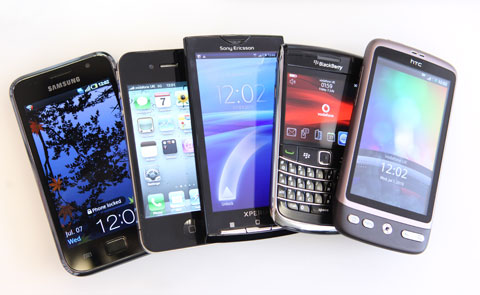
\includegraphics[width=0.6\textwidth]{smartphones.jpg}
   
   \vspace{0.5cm}

   \hrule
   {\size{32pt} \bfseries \scshape Smartphones}
   \vspace{1em}
   \hrule

   \vspace{0.5cm}

   {\Large \scshape Paper Computerarchitectuur en Netwerken}

   \vspace{2cm}

   \begin{minipage}{0.4\textwidth}\begin{flushleft}
      \large
      \begin{tabular}{rl}
      \multicolumn{2}{c}{\emph{Auteurs:}}\\
      Stefan  & \textsc{Kraaikamp}\\
      Edo     & \textsc{Mangelaars}\\
      Jurre   & \textsc{Smits}\\
      Maarten & \textsc{Staats}\\
      Erik    & \textsc{de Vries}
      \end{tabular}
   \end{flushleft}\end{minipage}
   \begin{minipage}{0.4\textwidth}\begin{flushright}
      \large
      \begin{tabular}{rl}
      \multicolumn{2}{c}{\emph{Docent:}}\\
      Lennart & \textsc{Herlaar}
      \end{tabular}
   \end{flushright}\end{minipage}

   \vfill

   Oktober 2012

\end{titlepage}

\begin{abstract}

De eerste telefoon die door het grote publiek `smartphone' werd genoemd was de Iphone uit 2007. Sindsdien is er een grote variatie ontstaan, maar smartphones worden allen gekenmerkt door extra functionaliteiten die de telefoon op een mini-computer laten lijken. In de architectuur van de smartphone is gekozen voor processoren en verbindingen die weinig ruimte en energie gebruiken. Dit zorgde voor een lagere complexiteit maar ook minder rekenkracht. De bekenste bestuuringssystemen zijn Android, iOS, Windows Windows Phone/Mobile en Symbian. Ze zijn voornamelijk aanpassingen van bestaande besturingssystemen voor computers. Ze verschillen in ontwikkelingstaal en focus op invoer, maar zijn allen gemaakt om met weinig resources zoveel mogelijk te doen. Gebruikersinteractie via de User Interface kenmerkt zich door het veelvuldig gebruik van een touchscreen en versnellingsmeter. Hierdoor zijn, naast toetsenbord en trackpad, ook touch en het draaien van het toestel mogelijkheden voor invoer van smartphones. Door visuele en fysieke feedback is het mogelijk op een klein scherm toch veel functionaliteiten te plaatsen. Omdat veel mensen de smartphone als mini-computer met bebehorende gevoelige informatie gebruiken, is het van belang om data goed te beveiligen. Dit gebeurt via functionaliteiten die in het besturingssysteem zijn ingebouwd maar ook via extra software(functionaliteiten). Deze beveiligingsmethoden richten zich vooral door inbreuk via netwerken. Daarnaast wordt in smartphones gebruik gemaakt van pincodes en beveiligingspatronen om fysieke inbreuk te voorkomen.

\end{abstract}


\tableofcontents

\chapter{Voorwoord}

Dit verslag is tot stand gekomen door een samenwerking van studenten van de Universiteit Utrecht. Voor het vak ``Computerarchitectuur en Netwerken'' is een beschrijvend verslag geschreven over de computerarchitectuur van smartphones. Wij willlen graag Lennart Herlaar bedanken voor het bijbrengen van de basiskennis van computerarchitectuur die we goed hebben kunnen gebruiken in dit verslag. Daarnaast willen we graag Wishnu Prasetya bedanken voor de hulp bij het zelf toepassen van de opgedane kennis.

De taakverdeling binnen dit verslag was als volgt: De samenvatting, voorwoord, introductie en geschiedenis zijn geschreven door Maarten Staats. Het stuk over de architectuur is geschreven door Edo Mangelaars. Het stuk over de bestuuringssystemen is geschreven door Stefan Kraaijkamp. Het stuk over de User Interface is geschreven door Juree Smits en het stuk over beveiliging en privacy is geschreven door Erik de Vries. Tenslotte is de conclusie geschreven door Maarten Staats.

Wij wensen u veel leesplezier,

Stefan Kraaikamp\\
Edo Mangelaars\\
Jurre Smits\\
Maarten Staats\\
Erik de Vries\\

\chapter{Introductie}

Hoewel enige tientallen jaren geleden ze nauwelijks een rol speelden, zijn mobiele telefoons hedendaags niet weg te denken uit de maatschappij.
Tegenwoordig is het niet alleen van belang dat je met een mobiele telefoon in staat bent om overal een telefoongesprek te kunnen voeren, maar worden veel hogere eisen aan mobiele telefoons gesteld, zoals hoge resolutie camara's, touchscreens, draadloos internet en vooral de mogelijkheid tot apps, kleine programma's die uiteenlopende services aanbieden.
Dit soort mobiele telefoons, die naast telefoongesprekken uitgebreidere computerfuncties aanbieden, noemen we smartphones.
De laatste jaren hebben smartphones de overhand gekregen op reguliere mobiele telefoons, van de totale verkoop van mobiele telefoons in het tweede kwartaal van 2012 was het aandeel van smartphones 66 procent \citep{GsmHelpDesk}.
Vanuit het oogpunt van de informatica is dit een interessante ontwikkeling, omdat smartphones zich steeds meer lijken te ontwikkelen tot mini-computers met bijbehorende funcationaliteiten.
Maar is de software architectuur in de smartphone net zo ontwikkeld als in bestaande computers?
Hoe gaan smartphone ontwikkelaars om met de beperking aan fysieke ruimte?
En wat is de invloed van de gebruikerinteractie door middel van een touchscreen?
Dit onderzoek zal zich richten op deze vragen.
Er wordt geprobeerd een beeld te schetsen over de architectuur binnen een smartphone en de randverschijnselen die daarbij horen.
De centrale onderzoeksvraag is: 

Hoe ziet de software architectuur van een smartphone eruit en wat betekent dit voor de gebruiker?

Om deze vraag te beantwoorden zal er gebruik gemaakt worden van de volgende deelvragen:

\begin{itemize}
   \item Hoe ziet de algemene software architectuur van de smartphone eruit en hoe verhoudt deze zich tot de architectuur binnen een normale computer?
   \item Van welke Operating Systems maakt de smartphone gebruik en hoe verschillen deze?
   \item Wat is de invloed van gebruikersinteractie via een touchscreen en hoe is deze terug te vinden in de applicaties?
   \item Hoe wordt in de software architectuur rekening gehouden met privacy en beveiliging?
\end{itemize}

In de rest van dit paper zullen deze vragen beantwoord worden.
Eerst zal kort de geschiedenis en de totstandkoming van de smartphone behandeld worden.
Daarna zal er gekeken worden naar de algemene structuur van de software architectuur.
Vervolgens zullen de meest gebruikte Operating Systems van de smartphone besproken worden.
Ten vierde zal de invloed van de gebruikerinteractie op de architectuur behandeld worden.
Daarna volgt de invloed van privacy en beveiliging op de architectuur.
En ten slotte zal er in de conclusie een antwoord worden gegeven op de onderzoeksvraag.

\chapter{Geschiedenis}

Het is 17 juni, 1946.
In St. Louis, een plaatsje in Missouri, Amerika, wordt ge\"experimenteerd met een technology die de wereld zal veranderen.
Vanuit zijn truck pleegt de bestuurder het eerste mobiele telefoongesprek \citep{ATnT}.
Vanaf dat moment gaan de ontwikkelingen snel.
Al twee jaar later is in veel steden en drukke plaatsen mobiele telefonie mogelijk.
De telefoons waren op dat moment nog log en waren ingebouwd in een auto en de plaatsen waar mobiel gebeld kon worden waren zeer beperkt vergeleken met nu.
Pas in 1969 kwam de eerste echte `mobiele telefoon' op de markt, in de vorm van een koffer.
In decenia die volgden werd de omvang van de telefoons steeds kleiner maar het gebied waarin gebeld kon worden steeds groter \citep{Farley}.

Vanaf 1990 begon de mobiele telefoon steeds vanzelfsprekender te worden in het dagelijks leven.
Hoewel vaak de iPhone als eerste echte smartphone wordt aangewezen, werd rond deze tijd al een eerste vorm van smartphone op de markt gezet in de vorm van IBM's Simon.
Deze telefoon, gei\"introduceerd in 1992, maakte gebruik van een touchscreen en was in staat voorspellend tekst aan te vullen.
Deze functies werden door de producenten aangeduid als `smart', vandaar de naam smartphone, hoewel deze naam pas 10 jaar later voet aan de grond zou krijgen \citep{BusinessWeek}.

Door de introductie van de iPhone ontstaat er een nieuw tijdperk in de ontwikkeling van de smartphone.
De iPhone, ge\"introduceerd in 2007, was de eerste smartphone die door een grote groep consumenten werd geadopteerd \citep{Hall}.
De eerste iPhone bevatte dan ook een enorme reikwijdte aan functies, zoals een mp3 speler, digitale camara, milti-touch en wi-fi internet connectie.
Daarnaast had deze iPhone extra features die `smart' genoemd kunnen worden, zoals energy saving licht sensor, versnellingsmeter en zoomfuncties bij o.a. foto's \citep{MacWorld}.
De standaard in de industrie voor smartphones is dan ook te herleiden op de eerste iPhone, die in feite geen telefoon meer was, maar een kleine computer met de mogelijkheid om telefoonfuncties aan te roepen.


\chapter{Architectuur}

Hoewel een smartphone in essentie een computer is, wijken de vereisten aan zowel de hardware als de software af van die van een PC.

Ten eerste moet een smartphone niet te groot zijn om in een broekzak te passen, waardoor de grootte van de componenten beperkt is, en in de gebruikersinterface rekening moet worden gehouden met de beperkte grootte van het scherm.
Hierdoor moet ook een keuze worden gemaakt voor het invoermechanisme van het apparaat tussen de combinatie van een gewoon scherm en een toetsenbord of `keypad' (een kleiner, toetsenbordje zonder lettertoetsen), een aanraakscherm of de combinatie aanraakscherm en een (al dan niet uitklapbaar) toetsenbord.
Ten tweede is de batterijcapaciteit begrensd door de grootte en de kosten van de batterij.
Dit heeft grote gevolgen voor zowel de software als de hardware die is toegepast om toch een zo groot mogelijk batterijleven te behouden.
Ten derde mag de warmteproductie niet te hoog zijn, aangezien de koelingscapaciteiten worden begrensd door het feit dat geen grote ventilatoren of heatsinks kunnen worden toegepast en het apparaat enigszins water- en stofdicht moet blijven.

Als laatste moet een smartphone uiteraard ook beschikken over de hardware om met behulp van een SIM-kaart met het mobiele-telefonienetwerk en eventuele WiFi-netwerken te communiceren. Voor deze communicatie bestaan veel standaarden, waarbij voor oude feature phones vooral de GSM-standaarden worden gebruikt en voor smartphones zowel GSM als (in recentere smartphones) 3G (3\textsuperscript{e} generatie), een technologie die snellere verbindingen aanbiedt, wordt gebruikt.


\section{Hardware}

\subsection{Processorarchitectuur}

Zoals genoemd is hitteproductie en energieverbruik een belangrijke factor in de keuze voor de processoren in smartphones, waardoor traditionele CISC- (Complex Instruction Set Computer) architecturen minder geschikt zijn voor deze apparaten.
Waar in PC's gestreefd wordt naar een zo hoog mogelijke rekenkracht is in mobiele apparaten een een afweging tussen rekenkracht en energieverbruik noodzakelijk.
Daarom wordt voor smartphones vrijwel altijd gekozen voor RISC- (Reduced Instruction Set Computer) processoren.

Waar in de PC-markt Intel de leider is in processorleveranciers vormt in meer dan 95\% van de mobiele telefoons van vandaag een ARM-processor het hart. Ongeveer de helft van de processoren die door ARM Holdings worden gemaakt komt terecht in mobiele computers en telefoons. \citep{economistarm}

Het verschil in CISC- en RISC-architecturen zit in de aanpak van het ontwerp van de chip.
Voordat RISC-processoren populair werden werd in de processormarkt gestreefd steeds complexere berekeningen te kunnen uitvoeren, zodat programmeurs met minder instructies dezelfde taken konden uitvoeren, wat weer bevorderlijk was voor de prestaties.
Toen echter de markt voor mobiele apparaten opkwam realiseerde men zich dat het energieverbruik van een processor een veel grotere factor was dan bij PC's, en RISC-chips een betere keuze waren.
Deze chips hebben een kleinere instructieset en hebben voor operaties die geheugen addresseren of aanpassen aparte instructies. 
Dit zorgt ervoor dat de complexiteit van de chip drastisch omlaag gaat, verlaagt het aantal transistoren in de kern van de CPU en maakt pipelining van instructies makkelijker.
Dit zorgt op zijn beurt weer dat hogere klokfrequenties behaald kunnen worden zonder dat daar meer energie voor wordt gebruikt (en dus warmte wordt geproduceerd). \citep{stanfordrisc}

\subsection{System on a Chip}

Naast de RISC-ontwerpaanpak hebben ARM-chips daarnaast ook nog een aparte manier van het verspreiden van hun chips.
In tegenstelling tot bijvoorbeeld Intel, die zelf hun chips maken en verkopen, verkoop ARM Holdings alleen licenties voor de ontwerpen van hun processoren.
Deze worden dan door andere fabrikanten opgenomen in chips die op hun beurt weer worden gebruikt in apparaten.

Dit biedt ruimte voor zogenaamde ``System on a Chip''-architecturen (SoC).
Dit zijn chips die in \'e\'en component een CPU, GPU, snelle en langzame bus en een geheugencontroller integreren.
Daarnaast kunnen ze andere hardware integreren zoals netwerkcontrollers, dedicated videodecoderingshardware en RAM- of flashgeheugen.
Dit verlaagt de complexiteit en fabricatiekosten voor smartphonemakers, doordat veel componenten van een apparaat in \'e\'en productieproces kunnen worden gemaakt.
Voorbeelden van deze chips zijn de NVIDIA Tegra en de Qualcomm Snapdragon series.
Deze SoC-fabrikanten gebruiken ontwerpen van ARM om zelf de processoren te maken.

\section{Software}

Hoewel smartphones qua hardware en gebruik veel weghebben van PC's zijn er verschillen in het publiceren en gebruiken van software die verder gaan dan het verschil in terminologie: `apps' in plaats van `programma's'.

Het grootste verschil is dat de meeste apps gepubliceerd worden via een `App Store' van de fabrikant, in plaats van dat de ontwikkelaars zelf verantwoordelijk zijn voor het verspreiden van de software.
De controle over welke apps ge\"installeerd kunnen worden ligt hierdoor (in meer of mindere mate) bij de fabrikant, welke over het algemeen testprocedures zullen hebben voor gebruikers de app kunnen gebruiken.
Dit heeft tot gevolg dat de gemiddelde kwaliteit van het softwareaanbod hoger zal zijn, maar leidt er ook toe dat software die concurreert met diensten van de fabrikant of partners daarvan (zoals apps voor telefonie of muziekverkoop) de kans hebben niet verkocht te mogen worden.

Een ander verschil ligt in de beperkte multitasking die mobiele besturingssystemen gebruiken.
Met beperking tot het OS en enkele apps die toestemming hebben om in de achtergrond te draaien (zoals muziekspelers) wordt maximaal \'e\'en app tegelijk gedraaid op een smartphone.
Wanneer tussen apps wordt geswitcht vraagt het OS de app de huidige toestand op te slaan op het flashgeheugen, sluit deze af en start de nieuwe app, al dan niet met de vorige toestand uit het flashgeheugen.
Dit heeft als voordeel dat het batterijleven wordt verhoogd omdat apps in de achtergrond niet langer stroom kunnen vragen. \citep{extremetechmulti}

Daarnaast staan apps over het algemeen meer op zichzelf dan programma's in PC's.
Communicatie tussen apps gebeurt buiten bij het gebruik van de `deel'-functionaliteit nauwelijks.
Apps worden meestal uitgevoerd in een zogenaamde \emph{sandbox}, wat betekent dat bijvoorbeeld bestandssysteemtoegang wordt beperkt tot een bepaalde context die bij de app hoort.
Ook wordt functionaliteit beperkt tot waar de app tijdens de installatie permissie voor heeft gevraagd.
Dit heeft tot gevolg dat apps minder mogelijkheden hebben schade toe te brengen aan het besturingssysteem, andere apps of privacygevoelige gegevens te kunnen lezen, maar beperkt wel de functionaliteit die apps kunnen aanbieden.


\chapter{Besturingssystemen}

Voor computers is het besturingssysteem een essentieel onderdeel voor een werkend systeem. Zo ook bij smartphones, smartphones zijn in de basis een kleine pc dus is het logisch dat ze ook een besturingssysteem nodig hebben om te kunnen werken. Smartphones bestaan nog niet zo lang en daarom is er nog veel concurrentie tussen verschillende producenten van smartphone besturingssystemen.

De besturingssystemen zijn:

\section{Android}

Android is samen met iOS het grootste besturingssysteem voor een smartphone \citep{canalys}. De grootste aandeelhouder van Android is Google, nadat Google het had overgenomen van Android inc. Het besturingssysteem is gebaseerd op de kernel van Linux en de applicaties die voor Android gemaakt zijn zijn gemaakt met Java. Het besturingssysteem is grotendeels bedoeld om te bedienen door middel van touchscreen, maar ook met een toetsenbord en trackpad kan Android bestuurd worden. Android is gemaakt om gebruikt te worden op smartphones, maar in de loop van de tijd zijn daarbij ook tablets bij gekomen en er zijn ook computers waarop Android ge\"installeerd staat. Het besturingssysteem was eerst alleen ontwikkeld om op ARM-instructieset te werken, maar sinds Android 4.0 is Android gaan samenwerken met Intel om er voor te zorgen dat Android ook kan werken op het x86-instructieset \citep{pcmweb}. Android staat er om bekend dat er veel aangepast kan worden aan het besturingssysteem, dat kan omdat het besturingssysteem opensource is en het besturingssyteem laat veel toe. Fabrikanten van smartphones passen Android aan om verschillend te zijn van de andere fabrikanten en soms ook om Android te verbeteren. Er zijn ook verschillende community's die Android aan passen en die stellen ze dan beschikbaar aan het publiek, ze zorgen er ook voor dat de meeste smartphones geüpgrade kan worden naar een nieuwere versie, want de producenten van smartphones geven alleen hun topmodellen vaak updates \citep{gsmacties}. Het is bij Android ook mogelijk om applicaties buiten de play store om te installeren. Dat heeft tot gevolgen dat applicaties ook van het internet te halen zijn. Je kunt daardoor als developer van een applicatie er voor kiezen om je applicatie via andere wegen aan te bieden. Aan de andere kant zorgt het ook voor meer piraterij omdat de applicaties door onbevoegde gratis aangeboden kunnen worden. De mogelijkheid dat je buiten Android om applicaties te installeren word ook gebruikt om malware op Android telefoons te installeren zonder dat ze het door hebben. De Google play store(Android market) werd eerst niet door Google gecontroleerd op malware, maar dit hebben ze later wel toegevoegd\citep{zdnet}.


\section{iOS}

iOS is het besturingssysteem die Apple gebruikt voor zijn smartphones, ze zijn ook de enige die het gebruikt. iOS is het eerste besturingssysteem voor smartphones die alleen op gericht is om te besturen door middel van touch, dat zie je ook terug in het uiterlijk van iOS, want je hebt verschillende schermen waar je tussen kan switchen en die kan je vullen met icoontjes waarmee je applicaties kan opstarten\citep{computerworld}. In die tijd was dat revolutionaire en iOS is daardoor nu ook zeer populaire \citep{mysecondskin}. iOS is gebaseerd op Mac osx, dat is het besturingssysteem van Apple voor hun computers. De applicaties voor iOS worden geschreven in objectiv c. iOS was eerst aangekondigd voor de iPhone, de i in iOS staat ook voor iPhone, en later ook nog voor de IPodtouch, de IPad en ook de Apple tv. iOS is een gesloten systeem, je hebt weinig mogelijkheden om het besturingssysteem aan te passen en de applicaties die voor iOS ontwikkeld worden moeten aan bepaalde regels van Apple voldoen om in de app store te komen. Het is wel mogelijk om via andere manieren applicaties te installeren, maar dan moet je door middel van beveiligings problemen in iOS het besturingssysteem aan passen waardoor je extra mogelijkheden kan krijgen. In de app store van iOS zijn momenteel de meeste applicaties beschikbaar voor mobiele besturingssystemen. 

\section{Blackberry OS}

Blackberry OS is ontwikkeld door RIM en word ook door RIM gebruikt voor hun smartphones, de Blackberry. Voor het besturen van het besturingssysteem gebruikten ze eerst de trackwheel, daarna zijn ze gebruik van de trackpad gaan maken, ze gebruiken dat nu nog steeds maar nu is het op sommige smartphones van BlackBerry ook mogelijk om het te bedienen via het touchscreen. BlackBerry OS is vooral gericht op de zakelijke markt en daarom hebben ook de meeste BlackBerry onder het scherm een volledig toetsenbord zitten, zo kunnen zakelijke mensen die onderweg zijn snel een email typen. RIM heeft ook enterprise service voor zakelijk gebruik ontwikkelt, ze hebben dat ontwikkelt zodat gebruikers hun bedrijfsmail kunnen koppelen aan hun Blackberry. Ze hebben ook internet service zodat je gebruik kan maken van hun internet browser en hun mail applicatie.  als je een van de enterprise abonnement hebt dan gaat het verkeer ook via de mailservers van je bedrijf en dat is zakelijk interessant omdat het verkeer na de server versleuteld is\citep{webwereld}. Het is niet verplicht om op een van de twee diensten van Blackberry te abonneren, maar dan kan de gebruiker geen gebruik maken van de applicaties van Blackberry die verbinding maken met internet, want die verbindingen gaan via de server van RIM\citep{wikipedia}. Blackberry was de afgelopen jaren zeer populaire onder niet zakelijke gebruikers, omdat je met de Blackberry internet service de applicatie ping kon gebruiken, maar sinds de komst van whatsapp, wat goedkoper is dan de dienst van Blackberry, is de populariteit van Blackberry afgenomen\citep{consumentenbond}. Het Blackberry OS is gebaseerd op Java. In het begin had RIM geen winkel waar je de applicaties kon downloaden, maar ze boden wel de mogelijkheid om third party applicaties te downloaden en te instaleren.

\section{Windows Mobile en Windows Phone}

Windows Phone/mobile is ontwikkelt door Microsoft. Windows Phone is de opvolger van Windows mobile, maar ze zijn allebei gebaseerd op een versie van Windows CE, dat is een aangepaste versie speciaal van Windows voor mobiele apparaten. Met de komst van Windows Phone 8 is dat alleen anders, want die is gebaseerd op Windows NT, daar zijn ook de Windows versies voor de computer op gebaseerd. Windows phone word bestuurd door middel van touch en heeft net als de xbox360 en windows8 een interface met veel grote vlakken, Microsoft noemt het de metro interface. Microsoft maakt zelf geen smartphones voor het besturingssysteem, maar ze laten smartphone producten smartphones produceren \citep{nrc}. Microsoft stelt wel eisen aan de resolutie van het scherm en de hardware die de producenten gebruiken. De producenten proberen zich te onderscheiden door verschillende scherm grootte toe te passen, dezelfde processor op verschillende snelheid te clocken en verschillende designs toe te passen. Toen Microsoft over ging van Windows mobile naar Windows Phone waren de applicaties niet compatibel met elkaar, van Windows phone 7 naar 8 is dat wel het geval, maar de smartphones die op Windows Phone 7 draaien krijgen geen update naar Windows Phone 8\citep{tweakers}.
 
 
\section{Symbian}

Symbian is het besturingssysteem dat opgericht is door symbian foundation,  veel groten bedrijven doen mee met de foundation. De belangrijkste deelnemer van de foundation is Nokia, Nokia heeft ook de foundation overgenomen in 2008. Symbian werd door veel producenten van smartphones gebruikt, maar sinds de komst van Android zijn er veel smartphone producenten overgestapt naar Android \citep{nieuwemobiel}. Nokia was de laatste grote producent die symbian gebruikte, maar die zijn volledig overgestapt op Windows phone. Symbian is te besturen via trackpad, maar de het is ook mogelijk om het via touch te bieden. Symbian is gemaakt in C++ en de applicaties die je voor symbian kan maken zijn ook in C++ geschreven.


\chapter{User interface}

\section{Evolution}

Om goed te kunnen begrijpen hoe de user interface (UI) van de moderne smartphone tot stand is gekomen moet eerst terug gekeken worden naar de manier waarop de UI eerst opgebouwd is. Voordat het scherm ook nog eens een invoer was werd het user interface zo ontworpen dat deze goed te navigeren was met behulp van de 4 richting toetsen omhoog, links, beneden en recht. Dit betekende dat alle menu's gebaseerd moesten zijn op een directory/lijst type formaat zodat met weinig acties toch veel bestanden en acties bereikt konden worden. Het probleem met zo’n opbouw is dat het heel snel onduidelijk wordt waar alles te vinden is omdat alles verborgen is achter directory's en menu's. Om dit probleem te verhelpen moest een nieuwe manier van invoer komen die navigeren in grotere stappen kan verzorgen. De toevoeging van het Touch screen aan smartphones zorgde ervoor dat de navigatie door de UI op een totaal andere manier mogelijk was. De eerste telefoon die de moderne vorm van UI in smartphones gebruikte was de iPhone. Deze gebruikte het feit dat er met behulp van het Touch screen direct objecten op het scherm geselecteerd konden worden. Hierdoor kan er veel meer op een scherm en dus in een menu vertoond worden zonder dat het een eeuwigheid duurt om iets te selecteren dat helemaal onderin staat. Dit zorgde ervoor dat de UI in veel minder menu’s verdeeld hoefde te worden en er ook meer gefocust kon worden op het uiterlijk van de overgebleven menu’s. Het uiterlijk van de UI gaat sindsdien met sprongen vooruit en ook de functionaliteit wordt steeds beter.

\section{Design}

De functie van het user interface is om interactie tussen de gebruiker en het apparaat mogelijk te maken. Het moet er dus voor zorgen dat er mogelijkheden zijn om applicaties te kunnen openen en makkelijk te navigeren naar deze applicaties en instellingen. Ten eerste moet er gekeken worden naar hoe de user naar een applicatie komt en daarna pas naar hoe de applicatie geopend kan worden. In moderne smartphones met een touch screen word er op 2 verschillende manieren door de UI heen genavigeerd. Er kan gescrold worden door een menu waardoor deze meer waarden of objecten kan laten zien. In moderne smartphones wordt dit naast de bekende manier van naar beneden gaan in een lijst op nog een andere manier gedaan die beter bekend is als swipen. Dit swipen laat meestal de ``volgende pagina'' van het menu zien door naar links of naar rechts te slepen op het scherm en is eigenlijk gewoon een variant van scrollen. Naast deze manier van navigeren die binnen menu’s gebeurt moet er ook een manier zijn om van menu naar menu te gaan. Dit gaat meestal op dezelfde manier waarop applicaties geselecteerd worden en verschilt weinig van de oude manier in de UI. Het selecteren van objecten of starten applicaties gebeurt simpelweg door op de grafische representatie te drukken. Nadat deze functies mogelijk zijn kan gekeken worden naar de manier waarop alles mooi en duidelijk op het scherm te zien is. Het uiterlijk van een user interface is even belangrijk als de mogelijke functionaliteit die deze levert. Het is namelijk erg moeilijk om functies te gebruiken als deze onduidelijk staan op het scherm. Voor navigatie is het erg belangrijk dat alle objecten die op het scherm staan duidelijk van elkaar te onderscheiden zijn. In de moderne smartphone UI wordt dit gedaan door de objecten weer te geven met iconen en daaronder een benaming. Daarnaast moeten de overgangen van menu naar menu of applicatie mooi zijn. 

\section{Invoer}

Het touch screen levert een gigantisch aantal mogelijkheden voor de gebruiker om het user interface te gebruiken. Hierdoor kan deze manier van invoer gezien worden als de belangrijkste manier van invoer in moderne smartphones. Het touch screen wordt gebruikt om te navigeren in menu's, om objecten te selecteren, applicaties te starten en nog veel meer. Navigeren wordt voornamelijk gedaan door het bewegen op het scherm van boven naar beneden of andersom (scrollen) en door bewegen van links naar recht of andersom (swipen). Deze zijn beide invoermogelijkheden met maar een enkele vinger, terwijl het scherm meerdere vingers aan kan. Het gebruiken van twee punten levert de mogelijkheid om veel gebruikte functies zoals inzoomen en uitzoomen mogelijk te maken met een enkele actie. Deze mogelijkheden zorgen ervoor dat het gebruik  van het apparaat veel makkelijker gaat. De volgende invoer mogelijkheid die een touch screen levert is het gebruik van een virtueel toetsenbord. Deze mogelijkheid is erg belangrijk aangezien de meeste smartphones geen individueel toetsenbord meer hebben. Zodra de user interface detecteert dat toetsenbord invoer nodig is roept deze een simpel virtueel toetsenbord. Om het toetsenbord nog te kunnen gebruiken kunnen er maar weinig toetsen op het scherm vertoond worden en zijn er dus knoppen om een andere layout te laden.  Naast het touch screen is er nog een vaak over het hoofd geziene invoer mogelijkheid. Als het toestel gedraaid wordt draait het scherm op zo’n manier dat deze recht op staat.  De manier waarop de oriëntatie van het apparaat bepaald wordt is met behulp van een accelerometer, deze detecteert ook beweging en is daarmee dus ook een invoer mogelijkheid. Er kan bijvoorbeeld met behulp van een snelle beweging van het apparaat naar rechts terug gegaan worden naar het beginscherm . Er zijn zelfs nog meer mogelijkheden door het combineren van het touch screen en de beweging.  Nadat een actie uitgevoerd is moet er feedback zijn over wat deze actie betekend. 

\section{Feedback}

Er zijn meerde types feedback die geleverd kunnen worden aan de gebruiker om duidelijk te maken dat een actie uitgevoerd is. De belangrijkste hiervan is de visuele feedback die op het scherm te zien is. Het mooie aan visuele feedback is dat het direct duidelijk is op het scherm wat voor een actie er uitgevoerd gaat worden, zelfs als het nog niet uitgevoerd is. Bijvoorbeeld als in de apple iPhone UI een icoon aangeklikt wordt opent de UI deze link. Maar als het icoon langdurig aangeklikt wordt zonder los te laten gaat het icoon langzaam schudden om aan te geven dat de actie nu een ander effect heeft, in dit geval kan het icoon daarna verschoven/verplaatst worden. Deze simpele visuele feedback maakt het duidelijk dat dezelfde invoer een andere actie uitvoert.  Naast visuele feedback is een andere belangrijke feedback de fysieke feedback. Deze wordt voornamelijk gebruikt als een manier van directe feedback bij het gebruik van een virtueel toetsenbord. Als een toets ingedrukt wordt vibreert het apparaat om deze actie duidelijk te maken. Het is belangrijk om feedback te krijgen om fouten te ontdekken en voorkomen.




\chapter{Beveiliging en Privacy}

Doordat smartphones niet alleen maar als telefoon dienen, maar de functionaliteiten van een mini-computer bezitten is de bescherming van privacy een sterk toenemende prioriteit aan het worden. Wanneer de complexiteit van software toeneemt, neemt hiermee ook het aantal bugs en zwakke plekken hierin die kwaadwillende zouden kunnen uitbuiten \citep{portokalidis2010paranoid}. 

Beveiliging van smartphones bestaat uit twee facetten. De eerste is het beveiligen van dataoverdracht. Daarnaast mag de data die erop staat opgeslagen niet toegankelijk zijn voor andere personen dan de eigenaar. Uit een onderzoek van ``the Association of Independent Research Centres'' onder 1600 smartphonegebruikers bleek dat 90\% van de ondervraagden ook zakelijke informatie op het apparaat opslaat en dat 20\% van de respondenten wel eens een smartphone is verloren \citep{charles2011}.  

De meeste beveiliging zit in ingebouwd in het Operating System. Hierin zijn vaak verschillende beveiligingsmechanismen ge\"implementeerd zoals procesisolatie, filesysteempermissies en geheugenbescherming.  Daarnaast kunnen er in hogere software lagen nog andere vormen van beveiliging ge\"implementeerd worden. Voorbeelden hiervan zijn: 

\begin{itemize}
   \item Antivirusprogramma's
   \item Firewalls
   \item Visuele notificaties
   \item Implementatie van een Turing test
\end{itemize}

\emph{antivirusprogramma's} zijn programma's die code analyseren en kwaadwillende code hieruit kunnen filteren. Veel ontwikkelaars voor antivirusprogramma's op PC's, (zoals o.a. AVG, Kaspersky, Norton) hebben ook programma's specifiek voor smartphones ontwikkeld \citep{becher2009security}. 

\emph{Firewalls} monitoren het dataverkeer van een client, in dit geval een smartphone. Door te reguleren welke programma's met welke andere programma's contact mogen maken worden de mogelijkheden van virussen significant verminderd \citep{becher2009security}. Vaak zit een firewall ge\"implementeerd in antivirussoftware, maar er bestaat ook specifieke software voor. 

\emph{Visuele notificaties} zijn berichtgevingen aan de gebruiker over belangrijke ondernomen acties. Een voorbeeld hiervan is het weergeven van nummer wanneer er een uitgaande oproep plaatsvindt. Indien deze actie niet door de gebruiker zelf gestart is kan deze actie ondernemen om dit te stoppen en weet hij dat er iets mis is op zijn telefoon. 

\fig{captcha.png}{CAPTCHA (bron: \citep{von2003captcha})}
Een \emph{Turing test} is een test die origineel ontwikkeld werd om de kunstmatige intelligentie van machines te testen. Hiermee werd getest of onderscheid gemaakt kon worden tussen de antwoorden die zij gaven en de menselijke antwoorden. Wanneer dit niet het geval was waren zij voor de test geslaagd. Tegenwoordig wordt de Turing test ook gebruikt als beveiliging door deze in te zetten voor opdrachten waar vanuit gegaan wordt dat ze alleen door menselijke gebruikers opgelost kunnen worden. De meest gebruikte vorm hiervan is de CAPTCHA (zie Figuur \ref{captcha.png}), een test waarbij gebruikers getoonde letters van een afbeelding moeten invoeren \citep{von2003captcha}. Hierdoor kan met grote zekerheid worden vastgesteld dat een actie door de gebruiker zelf is ge\"initieerd in plaats van kwaadwillende software \citep{becher2011mobile}. 

Smartphones kunnen op verschillende manieren door kwaadwillenden worden aangevallen. De meest voorkomende zijn via:

\begin{itemize}
   \item WiFi
   \item MMS
   \item GSM-netwerk
   \item Browser
   \item Application store
\end{itemize}

Een aanval via \emph{WiFi} wordt gedaan door de communicatie tussen het toestel en het acces-point af te luisteren. Hierdoor kan informatie zoals wachtwoorden worden verkregen. Het nadeel hiervan is dat hierdoor niet alleen de beveiliging van de telefoon in geding is, maar die van het hele netwerk. Dit probleem is niet uniek voor smartphones maar geldt voor alle apparaten die verbinding met een access point maken.

Er zijn gevallen geweest waarin virussen door middel van \emph{MMS} een bericht naar andere telefoons sturen en met een virus als bijlage die zich vermomt als filmpje of foto. Wanneer deze geopend wordt installeert deze zich op de telefoon en stuurt het zichzelf door naar alle contacten in de telefoon. 

Wanneer de encryptie van het \emph{GMS-netwerk} gebroken wordt kan alle communicatie van een smartphone worden afgeluisterd. 

Via een \emph{browser of application store} kunnen bestanden of programma's gedownload worden die schadelijk zijn. In tegenstelling tot de andere methoden worden deze vormen van verspreiding ge\"initieerd door de gebruiker en -- tenzij deze gecombineerd zijn met een worm -- zullen zij daarom minder snel grootschalig verspreid worden. 	

Om de fysieke toegang tot een telefoon te beperken hebben alle telefoons de mogelijkheid om de SIM-kaart met een pincode te beveiligen. Veel smartphones hebben tegenwoordig ook de mogelijkheid om voor de schermbeveiliging een patroon in stellen dat de gebruiker op het scherm moet tekenen om toegang tot de telefoon te krijgen. In gevallen waarbij de data extra privacygevoelig is kan er ook met biometrische identificatie, zoals een scan voor de ogen of handschriftherkenning. Een nadeel hiervan is echter dat om dit op een accurate manier te implementeren er grote investeringen in de hardware gedaan moeten worden. Hierdoor wordt deze laatste manier niet veel gebruikt \citep{thirumathyam2010}.  




\chapter{Conclusie}

Het begin van de mobiele telefonie is te herleiden op de tweede wereldoorlog. Rond 1990 werd de mobiele telefoon steeds vanzelfsprekender en rond die tijd is ook de eerste vorm van een smartphone op de markt gebracht. De eerste telefoon die onder het grote publiek bekendheid kreeg als `smartphone' was de eerste iPhone uit 2007. Sindsdien is de telefoon steeds verder ontwikkeld tot de `smartphone' die we nu kennen en de features die we erbij verwachten.

De architectuur van de smarthphone lijkt in het algemeen erg op die van een computer. Door andere eisen aan de smartphone, zoals klein formaat, beperkte grootte van het scherm en beperkte batterijcapaciteit, zijn er echter wel consessies gedaan aan functionaliteiten in de smartphone. Zo is de keuze gemaakt voor Reduced Instruction Set Computer (RISC) processoren, die minder energie gebruiken en minder hitte produceren. Daarnaast is de architectuur van het systeem een stuk kleiner gemaakt door gebruik van System on a chip (SoC) –architecturen. Deze combineren CPU, GPU, bussen en geheugencontroller in één chip. Ook andere hardware kan geïntegreerd worden, wat zorgt voor een reductie van complexiteit en ruimtegebruik. In het uitvoeren van software is met dezelfde eisen rekening gehouden. Zo mag er, enkele uitzonderingen daargelaten, maximaal \'e\'en app tegelijk draaien en beslaat de UI van een app het gehele scherm. Vergeleken met PC's is de manier waarom software (apps) gepubliceerd wordt erg beperkt. In de meeste besturingssystemen heeft de fabrikant controle over welke apps gepubliceerd worden. Dit heeft voordelen voor de veiligheid van het systeem en de kwaliteit van het softwareaanbod maar beperkt de functionaliteit die apps kunnen bieden.

Ook de besturingssystemen zijn afgeleid van normale computers, maar speciaal voor smartphones aangepast. Op dit moment is de Android het meest voorkomende besturingssysteem voor smartphones. Android maakt gebruik van een Linux kernel en applicaties in Java. Android geeft een hoge mate in vrijheid als het gaat om aanpassingsvermogen van het bestuuringssysteem. Dit in tegenstelling tot iOS, gebaseerd op Mac OS X, het besturingssysteem voor de iPhone. Applicaties in iOS hebben strenge regels waar ze aan moeten voldoen en applicaties kunnen alleen vanuit de App store geïnstalleerd worden. De iOS is speciaal ontwikkeld om alleen te besturen door middel van touch, wat ook terug te zien is in het uiterlijk van iOS smartphones. Blackberry OS, ontwikkeld door RIM, wordt gebruikt op Blackberry telefoons. De meeste blackberry's hebben een volledig toetsenbord en een trackpad, waar de OS op gebaseerd is. Veel BlackBerry's zijn voor zakelijk gebruik, en dat is ook te zien aan de extra functionaliteiten die het OS biedt, zoals mailservice en versleuteld dataverkeer. Applicaties op de Blackberry zijn, net als bij de Android, gebaseerd op Java. Een andere, opkomende, OS voor smartphones is de Windows Phone/Mobile. De eerste versies van dit OS waren gebaseerd op Windows CE, een aangepaste versie speciaal voor mobiele apparaten. Sinds Windows Phone 8 is dit OS gebaseerd op Windows NT, waar ook computerbesturingssystemen op gebaseerd zijn. Windows Phone/Mobile wordt voornamelijk bestuurd door touch en maakt gebruik van grote aanraakvlakken. Een andere, minder bekende, OS is Symbian, een besturingsysteem dat vooral door Nokia werd gebruikt. Tegenwoordig gebruikt Nokia Windows Phone. Symbian gebruikt vooral besturing via een trackpad maar heeft ook touch functies. Sybian en bijbehordende applicaties zijn in C++ geschreven.

Naast de bestuuringssyetemen is er in de User Interface ook rekening gehouden met de andere eisen die gesteld worden aan een smartphone. Vanuit de normale mobiel is de User Interface altijd bestuurd met 4 richtingstoetsen. Tegenwoordig gebruiken bijna alle smartphones touchscreen, waarbij in minder handelingen meer gegevens bereikt kunnen worden. Het touch screen kan van boven naar beneden genavigeerd worden (scrollen) en van links naar rechts (swipen). Andere invoermogelijkheden zijn een toetsenbord, trackpad of het draaien van het toestel. Opstarten van applicaties gaat snel door op de bijbehorende grafische representatie te drukken. Door visuele feedback te geven aan de gebruiker zijn op een beperkt scherm meerdere functies mogelijk, zoals een trillend icoontje dat aangeeft dat het verplaatst kan worden. Ook door vibratie van het toestel kan er feedback aan de gebruiker gegeven worden. Voor navigatie is het user interface erg belangrijk, omdat het duidelijk moet zijn welke functie zich waar bevindt, hier wordt bij smartphones dan ook veel aandacht aan besteed. 

Omdat men de smartphone tegenwoordig vaak gebruikt als minicomputer is privacy en beveiliging ook erg van belang. Beveiling van een smartphone bestaat uit het beveiligen van de data op de smartphone en het beveiligen van de dataoverdracht. Beveiliging zit vaak al in het OS ingebouwd, zoals proces isolatie, filesystem permissions en geheugenbescherming. Daarnaast zijn er hogere softwarelagen die gebruikt worden voor beveiliging, zoals antivirus programma's, firewalls, visuele notificaties en de Turing test, een test om te kijken of de gebruiker een machine of een mens is (bijvoorbeeld CAPTCHA). Deze softwarelagen beschermen tegen kwaadwillenden door aanvallen uit externe bronnen tegen te houden, zoals WiFi, MMS, de browser en applicaties. Bescherming tegen andere gebruikers die fysiek data van de telefoon willen halen, gebeurd via pincodes op simkaart en telefoon. Tegenwoordig wordt als schermbeveiliging van de telefoon vaak een patroon gekozen die de eigenaar op de telefoon moet tekenen, omdat dit makkelijker te onthouden is voor mensen.


\bibliographystyle{plainnat}
\bibliography{maarten1,edo,stefan,jurre,erik,maarten2}

\end{document}
